\documentclass[12pt]{article}
\usepackage[hmargin=3cm,vmargin=3.5cm]{geometry}

\usepackage[utf8]{inputenc}
\usepackage[french]{babel}
\usepackage[T1]{fontenc}
\usepackage{lmodern}

\usepackage{xcolor}
\usepackage{graphicx}
\usepackage{float}
\usepackage{amsmath}

\usepackage[justification=centering]{caption}

\graphicspath{ {F:/Travail/2A SRI\Identification paramétrique/TP_Identification_param/} }

\title{Compte rendu de TP\\ \textbf{Identification du modèle d'un système par la méthode des moindres carrés}}
\author{Fleytoux Yoann , Aurélien Bernier Levalois}
\date{11 octobre 2016}


% Document
\begin{document}
\maketitle


% Table des matières
\tableofcontents
\vspace{0.6cm}


\section{Présentation du TP}

L'objectif de ce TP est d'utiliser la méthode des moindres carrés, dans le contexte de l'automatique. Il s'agira ici d'identifier les paramètres du modèle d'un système dynamique donné. Pour cela, on sollicitera ce système avec une entrée connue et on observera ses sorties. Après avoir modélisé le problème, on appliquera la méthode des moindres carrés pour retrouver la meilleure valeur des paramètres compte tenu des entrées et sorties mesurées.


\section{Identification d'une fonction de transfert à pôles et zéros inconnus}
On considère ici un système dynamique préalablement modélisé. Cette modélisation a permis d'établir que ce système est d'ordre 3. Il peut donc être caractérisé par la fonction de transfert ci-après:
\smallbreak
\begin{math}
H(p)=Y(p)/U(p)=N(p)/D(p)=(ap^3+bp^2+cp+d)/(p^3+\alpha p^2+\beta p + \gamma)
\end{math}
 
\subsection{Travail préparatoire}
Sachant que l'on peut identifier directement une fonction de transfert par la méthode des moindres carrés, on cherche dans un premier temps à adapter le modèle de manière à pouvoir appliquer cette technique. Pour cela, on effectue les étapes suivantes:\smallbreak
\medbreak
\textbf{1.}En écrivant le produit en croix $D(p)Y(p)=N(p)U(p)$, montrer que:\smallbreak

\begin{math}
Y(p)=U(p)(a+b/p+c/p^2+d/p^3)-Y(p)(\alpha /p +\beta /p^2 + \gamma /p^3)
\end{math}

\smallbreak
\textbf{Réponse:}
\smallbreak
On sait que $N(p)=ap^3+bp^2+cp+d$ et que $D(p)=p^3+\alpha p^2+\beta p + \gamma$
\smallbreak
Si on remplace dans $D(p)Y(p)=N(p)U(p)$, on obtient:
\smallbreak
\begin{math}
Y(p)(p^3+\alpha p^2+\beta p + \gamma)=U(p)(ap^3+bp^2+cp+d)
\end{math}
\smallbreak
On divise par $p^3$ des deux côtés:
\smallbreak
\begin{math}
Y(p)(1+\alpha /p+\beta /p^2 + \gamma /p^3)=U(p)(a+b/p+c/p^2+d/p^3)
\end{math}
\smallbreak
On soustrait $Y(p)(\alpha /p+\beta /p^2 + \gamma /p^3)$ des deux côtés:
\smallbreak
\begin{math}
Y(p)=U(p)(a+b/p+c/p^2+d/p^3)-Y(p)(\alpha /p+\beta /p^2 + \gamma /p^3)
\end{math}
\medbreak
\textbf{2.} Prendre la transformée de Laplace inverse de l'expression précédente et montrer que le modèle possible de y(t) est donné par:
\smallbreak
\begin{math}
ymod(t)=\varphi ^T(t)P
\end{math}
\smallbreak
où $\varphi (t)$ est à déterminer et P le vecteur des paramètres à déterminer. $u(t)$ et $ymod(t)$ désignent respectivement la transformée de Laplace inverse de $U(p)$ et $Ymod(p)$. On précisera les dimensions de tous les termes.
\smallbreak
\textbf{Réponse:}
\smallbreak
%TODO trouver le nom de cette propriété
On utilise la propriété $X(p)/p = \int_{0}^{t} X(\tau) d\tau$:
\smallbreak
On sait que que :
\begin{math}
Y(p)=U(p)(a+b/p+c/p^2+d/p^3)-Y(p)(\alpha /p+\beta /p^2 + \gamma /p^3)
\end{math}
grace à la question 1. 
\smallbreak
En utilisant la propriété ,la transformée de Laplace inverse de $Y(p)$ devient donc:
\smallbreak
%\iint_V \mu(u,v) \,du\,dv
\begin{math}
L(Y(p))^-1=a U(t)
 +b \int_{0}^{t} U(\tau) d\tau 
 +c \int_{0}^{t} \int_{0}^{t} U(\tau) d\tau ^2 
 +d \int_{0}^{t} \int_{0}^{t} \int_{0}^{t} U(\tau) d\tau ^3
 -\alpha \int_{0}^{t} Y(\tau) d\tau
 -\beta \int_{0}^{t} \int_{0}^{t} Y(\tau) d\tau ^2
 - \gamma \int_{0}^{t} \int_{0}^{t} \int_{0}^{t} Y(\tau) d\tau ^3
\end{math}
\smallbreak
On met tout ça sous forme matricielle:
\smallbreak

$
\varphi _{7,1}(t) = 
 \begin{pmatrix}
U(t) \\
\int_{0}^{t} U(\tau) d\tau  \\
\int_{0}^{t} \int_{0}^{t} U(\tau) d\tau ^2 \\
\int_{0}^{t} \int_{0}^{t} \int_{0}^{t} U(\tau) d\tau ^3 \\
-\int_{0}^{t} Y(\tau) d\tau \\
-\int_{0}^{t} \int_{0}^{t} Y(\tau) d\tau ^2 \\
-\int_{0}^{t} \int_{0}^{t} \int_{0}^{t} Y(\tau) d\tau ^3 
\end{pmatrix}
$
et
$
P _{7,1} = 
 \begin{pmatrix}
a \\
b \\
c \\
d\\
\alpha \\
\beta\\
\gamma
\end{pmatrix}
$
\smallbreak
on a donc: $ 
ymod(t)=
\begin{pmatrix}
U(t) \\
\int_{0}^{t} U(\tau) d\tau  \\
\int_{0}^{t} \int_{0}^{t} U(\tau) d\tau ^2 \\
\int_{0}^{t} \int_{0}^{t} \int_{0}^{t} U(\tau) d\tau ^3 \\
-\int_{0}^{t} Y(\tau) d\tau \\
-\int_{0}^{t} \int_{0}^{t} Y(\tau) d\tau ^2 \\
-\int_{0}^{t} \int_{0}^{t} \int_{0}^{t} Y(\tau) d\tau ^3 
\end{pmatrix}^T(t)
*
\begin{pmatrix}
a \\
b \\
c \\
c\\
\alpha \\
\beta\\
\gamma
\end{pmatrix}
$
\medbreak
\textbf{3.} On suppose maintenant que l'on a effectué une expérience fournissant le vecteur de mesures suivant $Y=[y(t1),y(t2),...,y(tN)]^T$ où $k=1..N$ 
\smallbreak
\textbf{(a) } Exprimer $ymod(tk)$.
\smallbreak
\textbf{Réponse:}
\smallbreak:
\begin{math}
ymod(tk)=
\begin{pmatrix}
U(tk) \\
\int_{0}^{tk} U(\tau) d\tau  \\
\int_{0}^{tk} \int_{0}^{tk} U(\tau) d\tau ^2 \\
\int_{0}^{tk} \int_{0}^{tk} \int_{0}^{tk} U(\tau) d\tau ^3 \\
-\int_{0}^{tk} Y(\tau) d\tau \\
-\int_{0}^{tk} \int_{0}^{tk} Y(\tau) d\tau ^2 \\
-\int_{0}^{tk} \int_{0}^{tk} \int_{0}^{tk} Y(\tau) d\tau ^3 
\end{pmatrix}^T(tk)
*
\begin{pmatrix}
a \\
b \\
c \\
c\\
\alpha \\
\beta\\
\gamma
\end{pmatrix}
\end{math}
\smallbreak
\textbf{(b) } Déterminer les paramètres a,b et c qui minimisent le critère :
\smallbreak
\begin{math}
 J= \sum_{k=1}^{N} (y(tk)-ymod(tk))^2
\end{math}
\smallbreak 
\textbf{Réponse:}
\smallbreak
On pose $J=\varepsilon ^T \varepsilon$ avec:
\smallbreak
$
\varepsilon _{N,1} = 
 \begin{pmatrix}
y(t1) - ymod(t1) \\
y(t2) - ymod(t2) \\
... \\
y(tN) - ymod(tN)
\end{pmatrix}
$
\smallbreak
ce qui revient à:
\smallbreak
$
\varepsilon _{N,1} = 
 \begin{pmatrix}
y(t1)\\
y(t2)\\
... \\
y(tN)
\end{pmatrix}
-
\begin{pmatrix}
ymod(t1)\\
ymod(t2)\\
... \\
ymod(tN)
\end{pmatrix}
$
\smallbreak
or:
\smallbreak
$
\begin{pmatrix}
ymod(t1)\\
ymod(t2)\\
... \\
ymod(tN)
\end{pmatrix}
=
\phi_{N,7} P _{7,1}
$
\smallbreak
avec 
$\phi _{N,7}=
\begin{pmatrix}
\varphi _{7,1}(t1)^T\\
\varphi _{7,1}(t2)^T\\
... \\
\varphi _{7,1}(tN)^T
\end{pmatrix}
$
,
$
\varphi _{7,1}(tk) = 
 \begin{pmatrix}
U(tk) \\
\int_{0}^{tk} U(\tau) d\tau  \\
\int_{0}^{tk} \int_{0}^{tk} U(\tau) d\tau ^2 \\
\int_{0}^{tk} \int_{0}^{tk} \int_{0}^{tk} U(\tau) d\tau ^3 \\
-\int_{0}^{tk} Y(\tau) d\tau \\
-\int_{0}^{tk} \int_{0}^{tk} Y(\tau) d\tau ^2 \\
-\int_{0}^{tk} \int_{0}^{tk} \int_{0}^{tk} Y(\tau) d\tau ^3 
\end{pmatrix}
$
et
$ 
P _{7,1}=
\begin{pmatrix}
a \\
b \\
c \\
d\\
\alpha \\
\beta\\
\gamma
\end{pmatrix}
$
\smallbreak
On note:
$
Y _{N,1}=
 \begin{pmatrix}
y(t1)\\
y(t2)\\
... \\
y(tN)
\end{pmatrix}
$
\smallbreak
On a donc:
$
J=
( Y _{N,1} - \phi_{N,7} P _{7,1} )^T(Y _{N_1} - \phi_{N,7} P_{7,1})
$
\smallbreak
Or $(A B)^T = A^T B^T $ donc:
\smallbreak
$
J=
( Y _{N,1}^T - \phi_{N,7}^T P _{7,1}^T )(Y _{N_1} - \phi_{N,7} P_{7,1})
$
\smallbreak
On peut voir que J dépend explicitement de $P$, et donc de a,b et c. ATTENTION: pour la suite quand on les dimensions des matrices sont écrites avant la transposée (ex $A _{1,2}^T$ est une matrice de dimension 2,1 après la transposée. 
\medbreak
$
J=
Y _{N,1}^T Y _{N,1} -  Y _{N,1}^T \phi_{N,7} P _{7,1} - P _{7,1}^T  \phi_{N,7}^T Y _{N_1} + P_{7,1}^T \phi_{N,7}^T \phi_{N,7} P_{7,1}$
\smallbreak

Condition du 1er ordre: $\Delta j = 0$ 
\smallbreak
$
\Delta Y^T Y = d(Y^T Y)/dP = 0 _{N,1}
$
\smallbreak
$
\Delta (Y ^T \phi P) = d(Y ^T \phi P)/dP = \phi ^T Y 
$

\smallbreak
$
\Delta (P^T \phi ^T Y) =d(P^T \phi ^T Y)/dP= \phi ^T Y
$
\smallbreak
$
\Delta (P^T \phi ^T \phi P) =d(P^T \phi ^T \phi P))/dP
$
\smallbreak
$
= [ \phi ^T \phi + (\phi ^T \phi)^T]P
$
\smallbreak
$
= 2 \phi ^T \phi P
$
\smallbreak
Donc: $ \Delta J = 0 _{N,1} - \phi ^T Y - \phi ^T Y + 2 \phi ^T \phi P$
\smallbreak
Ce qui donne : $2 \phi ^T \phi P - 2 \phi ^T Y$
\smallbreak
Condition du 1er ordre: $\hat{P}$ est optimum si $\Delta J=0$ en $\hat{P}$
\smallbreak
Donc: 
$2 \phi ^T \phi P - 2 \phi ^T Y =0$
\smallbreak
$2 \phi ^T \phi P  =2 \phi ^T Y$
\smallbreak
$ \phi ^T \phi P  = \phi ^T Y$
\smallbreak
Estimateur des moindres carrés: 
$\hat{P}=(\phi ^T \phi)\up{-1} \phi ^T Y$
\smallbreak
\begin{math}
\hat{P}=(
\begin{pmatrix}
\varphi _{7,1}(t1)^T\\
\varphi _{7,1}(t2)^T\\
... \\
\varphi _{7,1}(tN)^T
\end{pmatrix} ^T
\begin{pmatrix}
\varphi _{7,1}(t1)^T\\
\varphi _{7,1}(t2)^T\\
... \\
\varphi _{7,1}(tN)^T
\end{pmatrix})\up{-1} 
\begin{pmatrix}
\varphi _{7,1}(t1)^T\\
\varphi _{7,1}(t2)^T\\
... \\
\varphi _{7,1}(tN)^T
\end{pmatrix} ^T 
\begin{pmatrix}
y(t1)\\
y(t2)\\
... \\
y(tN)
\end{pmatrix}
\end{math}
\smallbreak
Quel sens à ce critère?
\smallbreak
On cherche à minimiser l'erreur entre le système réel et celui  modélisé.


\subsection{Mise en oeuvre sous Matlab}
\smallbreak
\textbf{1.} Rappeler brièvement le principe de la méthode d'intégration des rectangles.
\smallbreak
\textbf{Réponse:} 
\smallbreak
La méthode d'intégration des rectangles permet de calculer l'intégrale d'une fonction en additionnant les aires des rectangles formant la courbe.
Cette aire est donc le produit du pas d'échantillonnage et de  la valeur de l'échantillon en un tk donné.
\smallbreak
En quoi la fonction cumsum sous matlab peut-elle être intéressante pour réaliser cette fonction d'intégration?
\smallbreak
\textbf{Réponse: }
\smallbreak
 B = cumsum(A) retourne la somme cumulée A partir du début de la première dimension du tableau A dont la taille est différente de 1.

    Si A est un vecteur, alors cumsum(A) renvoie un vecteur contenant la somme cumulée des éléments A.

En multipliant les échantillons par le pas d'échantillonnage, elle permettra de calculer la somme des aires des rectangles et donc réaliser l'intégration.
\medbreak
\textbf{2.}A l'aide de la fonction précédente, déterminer la valeur du vecteur de paramètres P sous matlab. Stocker la fonction de transfert estimée dans une variable sous matlab.
\smallbreak
\textbf{Réponse:}
\smallbreak
En exécutant ce code matlab, on obtient:

\begin{flushleft}
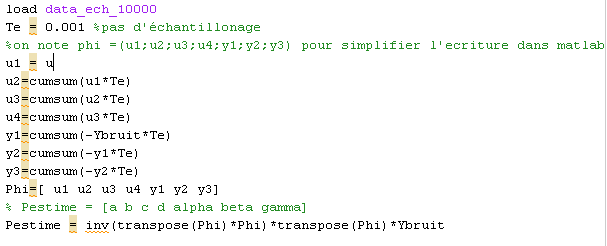
\includegraphics{2_2.PNG}
\end{flushleft}

$\hat{P}=
\begin{pmatrix}
0.4987\\
 4.1954\\
 3.2927\\
5.6041 \\
 4.9945\\
   -5.9935\\
   7.0058
\end{pmatrix}
$

\medbreak
\textbf{3.} Superposer la sortie du modèle aux mesures. Conclure quand à la qualité de l'identification.
\smallbreak
\textbf{Réponse:}
\begin{flushleft}
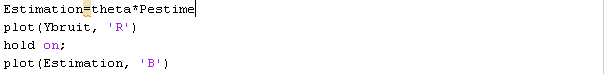
\includegraphics{2_3.PNG}
\end{flushleft}
Pour N=10000, avec en l'amplitude ordonnée et le numéro d'échantillon en abscisse.
\begin{flushleft}
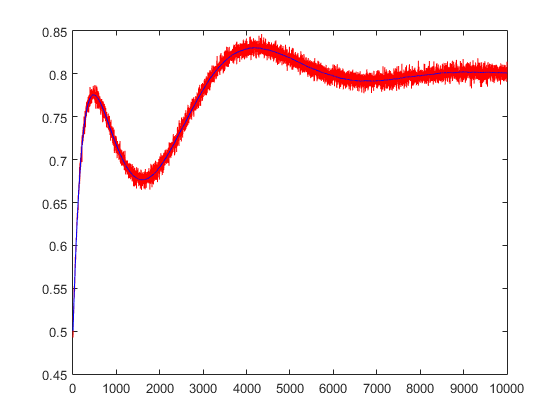
\includegraphics{2_3_graph}
\end{flushleft}
On a ici, en bleu le modèle estimé et en rouge ce que l'on a mesuré. On observe que la qualité de l'identification est bonne, la courbe bleue est juste lissée par rapport à la courbe mesurée (pas de bruit du aux mesures). 

\medbreak
\textbf{4.} On souhaite maintenant analyser l'impact du nombre de mesures prélevées sur la qualité de l'identification. Pour cela, on effectue une seconde expérience où l'on sollicite le système avec le même échelon, maintenant en prélevant seulement $N=50$ points.
\smallbreak
\textbf{(a)} Estimer les paramètres pour ce deuxième cas de figure et donner leur valeur.
\smallbreak
\textbf{Réponse:}
\begin{flushleft}
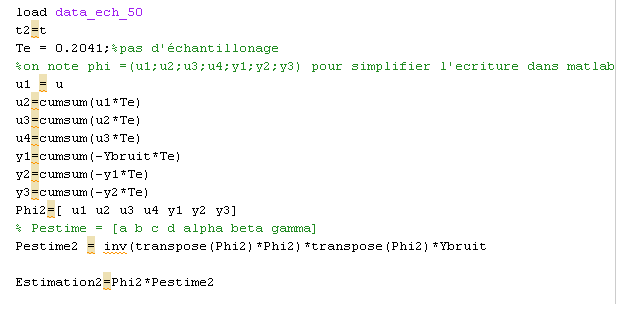
\includegraphics{2_4_a.PNG}
\end{flushleft}
$\hat{P}=
\begin{pmatrix}
  -0.0450\\
    6.0828\\
    2.3675\\
    8.8804\\
    6.6415\\
   -6.4200\\
   11.1065
\end{pmatrix}
$
\smallbreak
\textbf{(b)} Superposer maintenant les mesures et les sorties du modèle obtenues pour N=50 et N=1000 mesures. Conclure
\textbf{Réponse:}
\begin{flushleft}
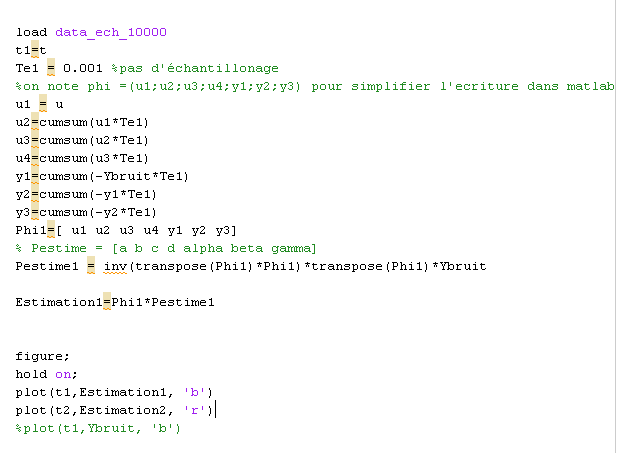
\includegraphics{2_4_a_2.PNG}
\end{flushleft}
Pour N=10000 en bleue et N=50 en rouge, avec en ordonnée l'amplitude et le temps en secondes en abscisse.
\begin{flushleft}
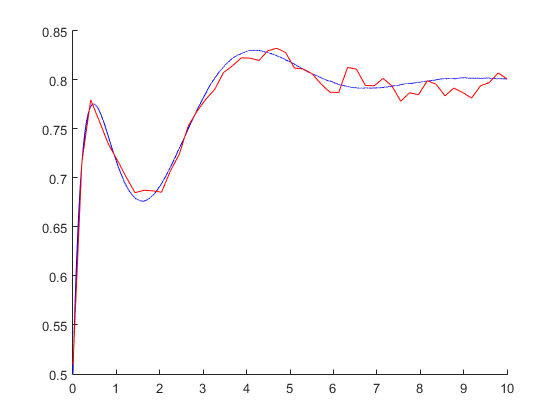
\includegraphics{2_4_b.PNG}
\end{flushleft}
Le modèle à 50 échantillons est moins précis que celui à 10000. Le nombre d'échantillons est donc un facteur déterminant de la qualité de l'identification.
\medbreak

\textbf{5.} Afin d'évaluer la validité de l'estimation, on effectue une dernière expérience où le système est sollicité avec une sinusoïde. Celle-ci est définie par la transformée de Laplace suivante:
\smallbreak
$
p/(p^2 + 1)
$
\smallbreak
Simuler la réponse du modèle obtenu précédemment avec la sinusoïde.
\smallbreak
\textbf{Réponse:}
\begin{flushleft}
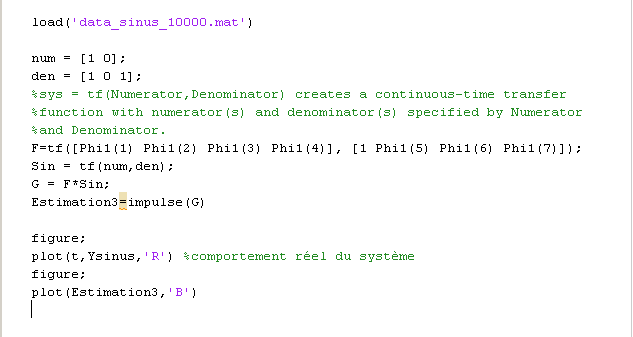
\includegraphics{2_5.PNG}
\end{flushleft}
\begin{flushleft}
Le système réel:
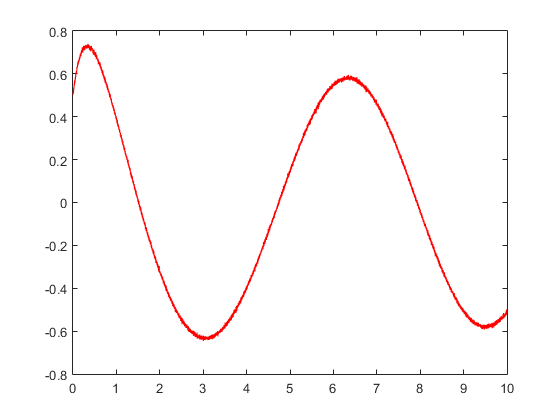
\includegraphics{Sin.PNG}
\end{flushleft}
La réponse à la sinusoïde du système modélisé précédemment:
\begin{flushleft}
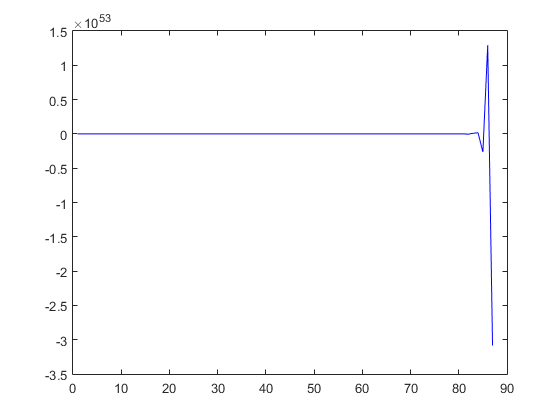
\includegraphics{Estimation_sin.PNG}
\end{flushleft}
Conclusion: Notre modélisation diverge, ce qui n'est pas le cas des mesures. 
\end{document}
 